\textbf{7-1.}一根长为 $l$ 的不均匀细杆, 其线密度 $\lambda = a + bx$ ( $x$ 为离杆的一端 $O$ 的距离。 $a, b$ 为已知常量)。求该杆对过 $O$ 端并垂直于杆的轴的转动惯量。

\vfill

\textbf{7-2.}一质量为 $m_0$ 、半径为 $R$ 的均质圆盘, 可绕过其圆心且垂直于圆盘的光滑水平轴在竖直平面内转动。在盘的边上绕有一不可伸长的细绳, 绳的一端连有一质量为 $m$ 的物体。开始时, 绳子被拉直, 物体 $m$ 的高度为 $h$ , 并由静止开始

下降,设绳与盘边之间无相对滑动。试求:

(1) 绳的张力 $F_{T}$ ;

(2) 物体 m 到达地面所需的时间 t。

\begin{figure}[H]
  \centering
  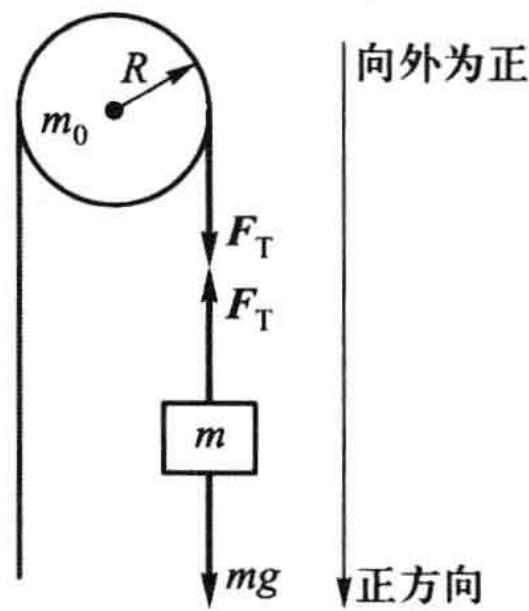
\includegraphics[width=0.25\textwidth]{figures/fig7-2.jpg}
  \end{figure}

\vfill
\newpage

\textbf{7-3.}在粗糙的水平面上,一半径为 $R$ 、质量为 $m$ 的均质圆盘绕过其中心且与盘面垂直的竖直轴转动,如习题 7-3 图所示。已知圆盘的初角速度为 $\omega_0$ ,圆盘与水平面间的摩擦因数为 $\mu$ ,若忽略圆盘轴承处的摩擦,问经过多长时间圆盘将静止?

\begin{figure}[H]
  \centering
  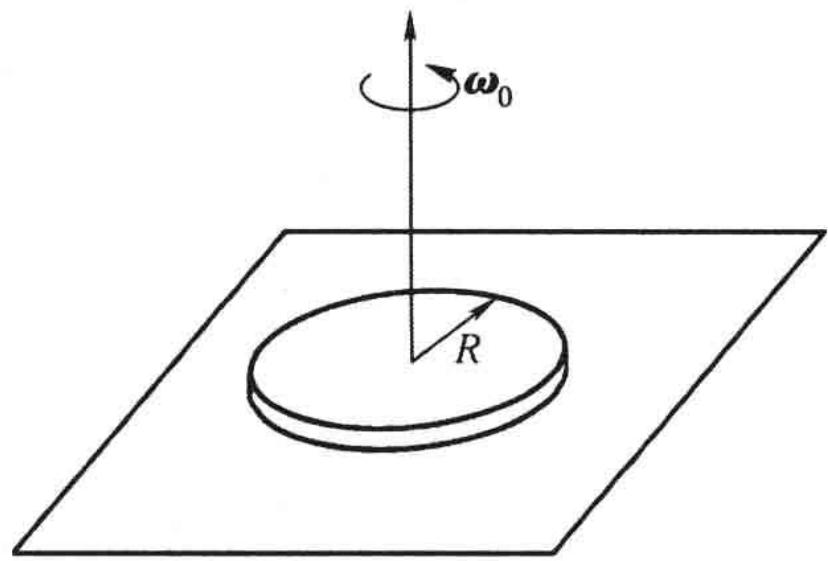
\includegraphics[width=0.3\textwidth]{figures/fig7-3.jpg}
  \end{figure}

\vfill

\textbf{7-4.}一个高为 $h$ 、底半径为 $R$ 的圆锥体, 可绕其固定的竖直轴自由旋转。在其表面沿母线刻有一条光滑的斜槽, 如习题 7-4 图所示。开始时, 锥体以角速度 $\omega_0$ 旋转, 此时, 将质量为 $m$ 的小滑块从槽顶无初速释放。设在滑块沿槽滑下的过程中始终不脱离斜槽，而锥体绕竖直轴的转动惯量为 $J_{0}$ 。试问：

(1) 当滑块到达底边时, 圆锥体的角速度为多大?

(2) 当滑块到达底边时, 滑块相对地面的速度为多大?

\begin{figure}[H]
  \centering
  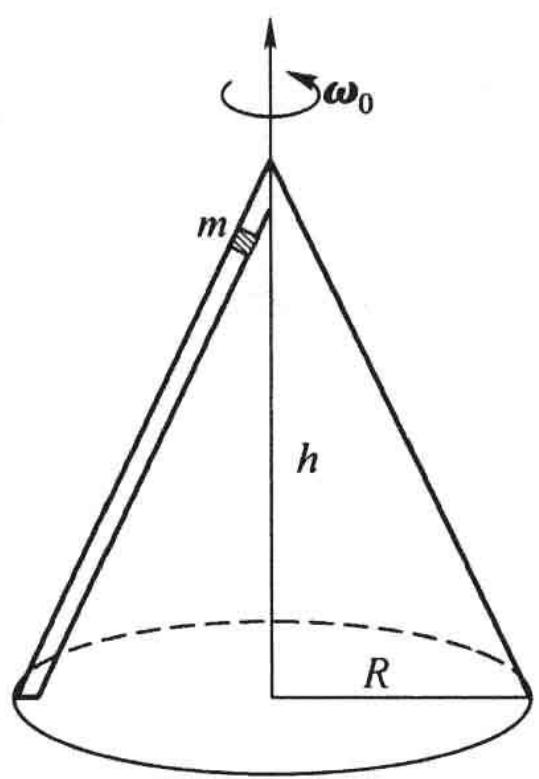
\includegraphics[width=0.2\textwidth]{figures/fig7-4_1.jpg}
  \end{figure}

\vfill
\newpage

\textbf{7-5.}质量为 $m$ 、半径为 $r$ 的均质球置于粗糙的水平面上, 球与水平面之间的摩擦因数为 $\mu$ 。开始时, 球的转动角速度为 $\omega_0$ 而质心静止。试问:

(1) 经过多长时间球开始做纯滚动?

(2) 球做纯滚动时质心的速度为多大?

\vfill

\textbf{7-6.}将一根长为 $L$ 、质量为 $m$ 的均匀杆上长为 $l\left(l < \frac{1}{2} L\right)$ 的一段搁在桌边，另一端用手托住，使杆处于水平状态，如习题 7-6 图所示。现释放手托的一端，试问，当杆转过的角度 $\theta$ 为多大时，杆开始滑离桌边（设杆与桌边之间的摩擦因数为 $\mu$ ）？

\begin{figure}[H]
  \centering
  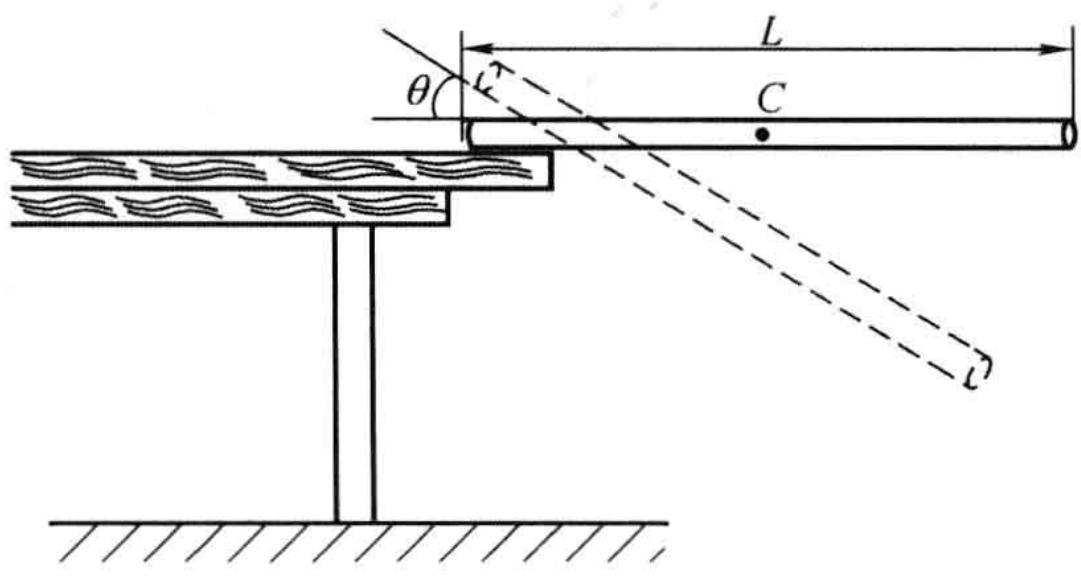
\includegraphics[width=0.4\textwidth]{figures/fig7-6.jpg}
  \end{figure}

\vfill
\newpage

\textbf{7-7.}质量为 $m$ 的子弹, 以速度 $v_{0}$ 射入质量为 $m_{0}$ 、半径为 $R$ 的圆盘的边缘, 并留在该处。 $v_{0}$ 的方向与入射处的半径垂直, 如习题 7-7 图所示。试就以下两种情况:

(1) 盘心装有一与盘面垂直的光滑固定轴;

(2) 圆盘是自由的。

求子弹射入后圆盘系统总动能之比 $E_{k1}/E_{k2}$ 。

\begin{figure}[H]
  \centering
  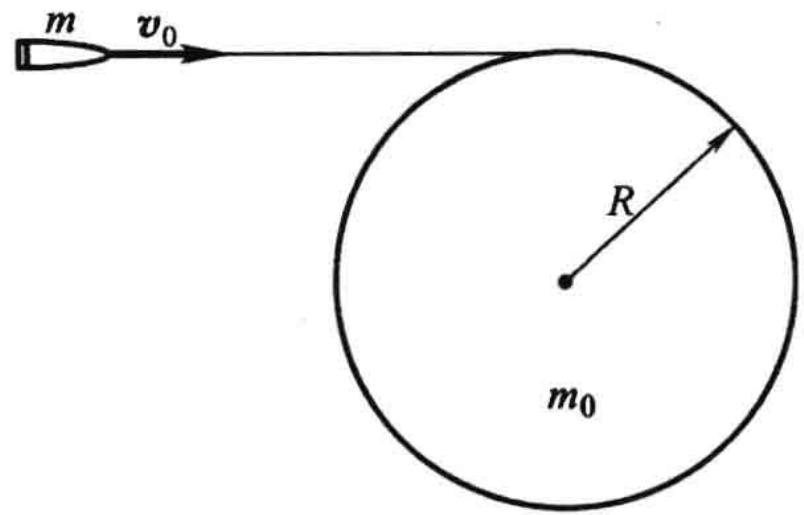
\includegraphics[width=0.3\textwidth]{figures/fig7-7_1.jpg}
  \end{figure}

\vfill

\textbf{7-8.}如习题 7-8 图所示, 质量为 $m_{0}$ 、半径为 $R$ 的弹性球在水平面上做纯滚

动,球心速度为 $v_{0}$ ,与粗糙的墙面发生碰撞后,以相同的球心速度反弹,设球与墙面、水平面的摩擦因数都为 $\mu$ , 碰撞时球与水平面的摩擦可以忽略。

（1）碰撞后，球经过一段时间开始做纯滚动，求此时的球心速度；

(2) 若球与墙面之间的碰撞时间为 $\Delta t$ , 为使碰撞时球不会跳起, 则摩擦因数应满足什么关系? 设碰撞过程中的相互作用力为恒力。

\begin{figure}[H]
  \centering
  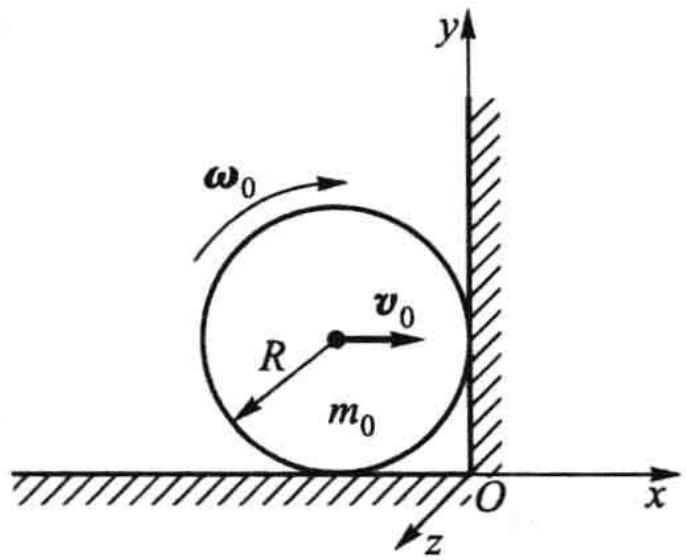
\includegraphics[width=0.33\textwidth]{figures/fig7-8.jpg}
  \end{figure}

\vfill
\newpage

\textbf{7-9.}一根长为 $2l$ , 质量为 $2m_0$ 的均匀细杆, 可以绕过中点的固定轴在水平面内自由转动。在离中心 $\frac{1}{3} l$ 处各套有两个质量均为 $m$ 的小珠子, 开始时杆的转动角速度为 $\omega_0$ , 而两小珠相对静止。当释放小珠后, 小珠将沿杆无摩擦地向两端滑动。试问:

(1) 当小珠滑至杆端时,杆的角速度为多大?

(2) 当小珠滑至杆端时, 小珠相对杆的速度为多大?

(3) 当小珠滑离杆时, 小珠的速度为多大?

\vfill

\textbf{7-10.}两根质量均为 $m$ 、长度均为 $l$ 的相同均质细杆 $AC$ 与 $CB$ , 两杆的 $C$ 端用一光滑的铰链相连。将两杆分开一定角度, 让 $A$ 、 $B$ 端与光滑地面接触, 并使两杆均在竖直平面内。开始时, 两杆与地面间的夹角均为 $\theta$ 。现无初速地释放两杆, 问两杆着地时 $C$ 点的速度。

\vfill
\newpage

\textbf{7-11.}两光滑墙面互相垂直, 在墙 B 上离墙面 A 距离 s 处, 有一光滑钉子,

将一长度为 2l、质量为 $m_{0}$ 的均匀杆的一端抵在墙上，杆身斜置在钉子上，使杆位于垂直于墙面 A 的竖直平面内，求平衡时杆与水平面所成的角 $\theta$ 。

\begin{figure}[H]
  \centering
  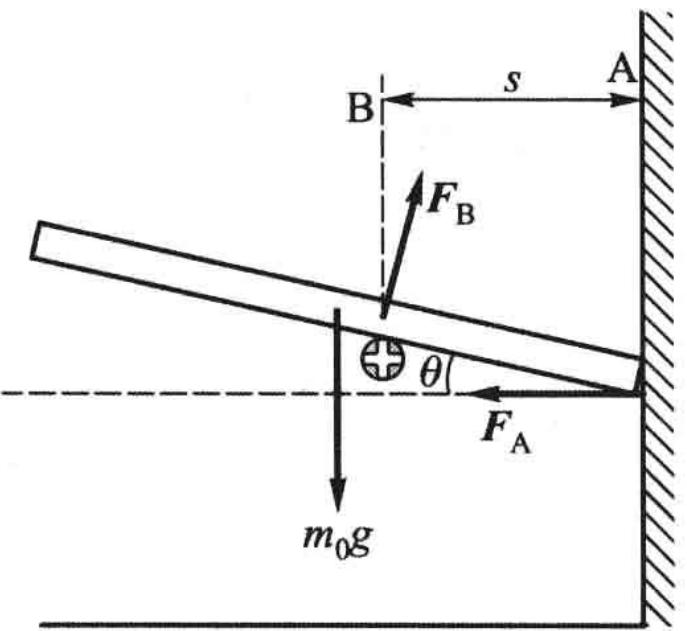
\includegraphics[width=0.25\textwidth]{figures/fig7-11.jpg}
  \end{figure}

\vfill

\textbf{7-12.}如习题 7-12 图所示, 一飞轮以 $\omega$ 的角速度高速转动, 其转动惯量为 $J_{0}$ , 试问, 为使水平圆台以恒定角速度 $\Omega$ 转动 ( $\Omega \ll \omega$ ), 则所需加在圆台上的力矩为多大?

\begin{figure}[H]
  \centering
  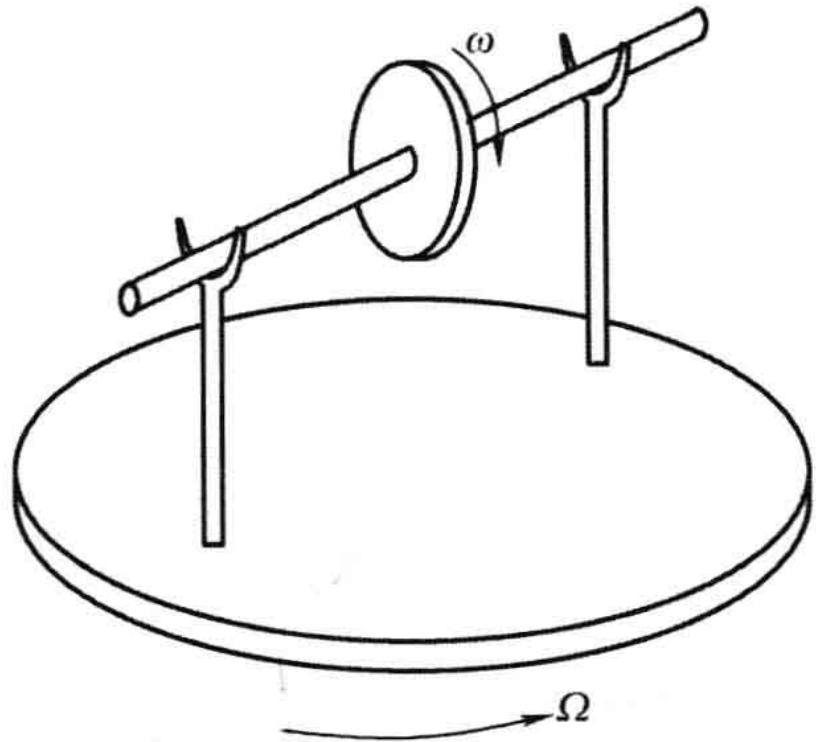
\includegraphics[width=0.25\textwidth]{figures/fig7-12.jpg}
  \end{figure}

\vfill
\newpage

\textbf{7-13.}在光滑水平面上, 质量均为 $m_{0}$ 的两小球由一长为 $l$ 的轻杆相连。另一质量为 $m$ 的小球以 $v_{0}$ 的速率向着与杆成 $\theta$ 角的方向运动, 并与某一 $m_{0}$ 发生碰撞, 碰后 $m$ 以 $\frac{1}{2} v_{0}$ 的速率沿原路线反弹。试求碰撞后轻杆系统绕其质心转动的角速度 $\omega$ , 参见习题 7-14 图。

\vfill

\textbf{7-14.}若上题中三球的质量相同, 均为 $m$ , 且 $\theta = 45^{\circ}$ 。当运动小球以 $v_{0}$ 的速率与连在杆上的某一球发生弹性碰撞后, 即沿垂直于原速度的方向运动, 如习题 7-14 图所示。试求:

(1) 碰撞后, 运动小球的速度 $v_{f}$ ;

(2) 碰撞后, 轻杆系统绕其质心转动的角速度 $\omega$ 。

\begin{figure}[H]
  \centering
  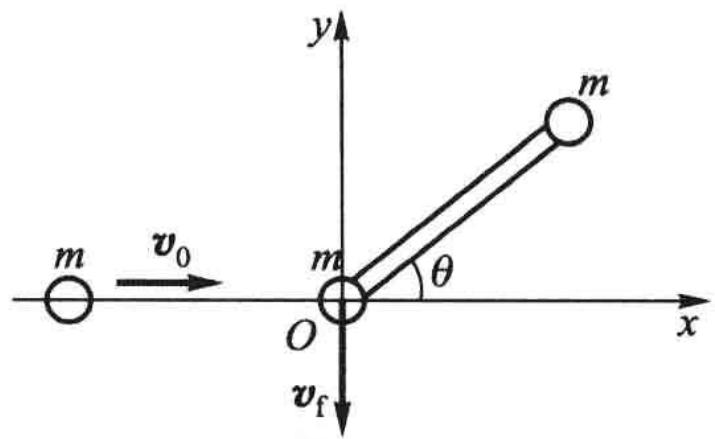
\includegraphics[width=0.4\textwidth]{figures/fig7-14.jpg}
  \end{figure}

\vfill
\newpage

\textbf{7-15.}一块边长为 $a$ 、质量为 $m_{0}$ 的正三角形薄板, 求该板对过其一边的轴的转动惯量。

\begin{figure}[H]
  \centering
  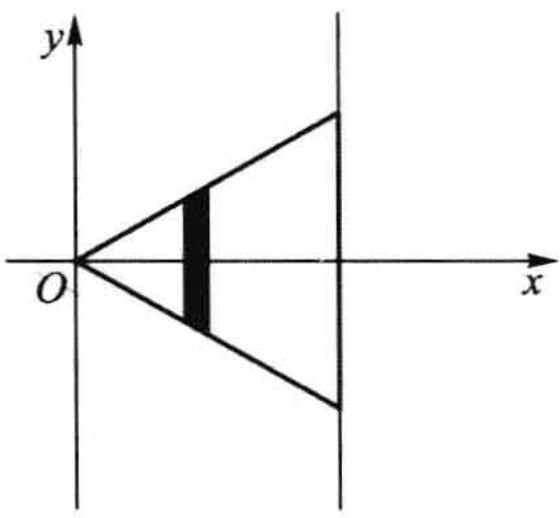
\includegraphics[width=0.3\textwidth]{figures/fig7-15.jpg}
  \end{figure}

\vfill

\textbf{7-16.}在质量为 $m_{0}$ 、半径为 $R$ 的匀质圆盘上, 有三个半径为 $\frac{1}{3} R$ 的小圆孔, 圆孔的圆心分别在三条半径的中心处, 此三条半径把圆盘分割成相等的三块, 如习题 7- 16 图所示。求此圆盘对过其圆心且与盘面垂直的轴的转动惯量。

\vfill
\newpage

\textbf{7-17.}两块质量均为 $m_{0}$ 、半径均为 $R$ 的均匀薄圆盘间连有一均匀细杆, 细杆长为 $l$ , 质量为 $m$ , 过两盘的圆心且与圆盘垂直, 如习题 7-17 图所示。求此装置对通过某一圆盘直径的轴的转动惯量。

\begin{figure}[H]
  \centering
  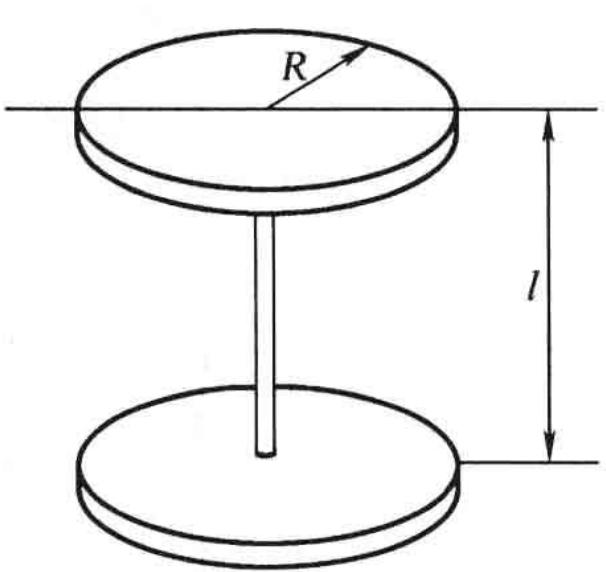
\includegraphics[width=0.25\textwidth]{figures/fig7-17.jpg}
  \end{figure}

\vfill

\textbf{7-18.}质量分别为 $m_{1} = 200 \mathrm{~g}, m_{2} = 250 \mathrm{~g}$ 的两个物体用细绳相连, 绳子套在质量 $m_{0} = 100 \mathrm{~g}$ , 半径 $r = 10 \mathrm{~cm}$ 的滑轮上, $m_{2}$ 放在光滑的水平桌面上, $m_{1}$ 悬挂着, 如习题 7-18 图所示。设滑轮为一质量均匀的圆盘, 绳子的长度不变, 绳子的质量及滑轮轴承处的摩擦均可忽略不计, 绳子与滑轮之间无滑动。求 $m_{1}$ 的加速度 $a$ 以及绳子各处的张力 $F_{\mathrm{T} 1}$ 和 $F_{\mathrm{T} 2}$ 。

\vfill
\newpage

\textbf{7-19.}如习题 7-19 图所示的阿特伍德机中, 两物体质量分别是 $m_{1}$ 和 $m_{2}$ ,

滑轮半径为 R，质量为 $m_{0}$ 。若物体运动时，滑轮与绳之间有相对滑动，两者之间的摩擦因数为 $\mu$ 。设绳不可伸长，忽略滑轮轴承处的摩擦。试求：

(1) $m_{1}$ 与 $m_{2}$ 的加速度；

(2) 滑轮的角加速度 $\alpha$ 。

\begin{figure}[H]
  \centering
  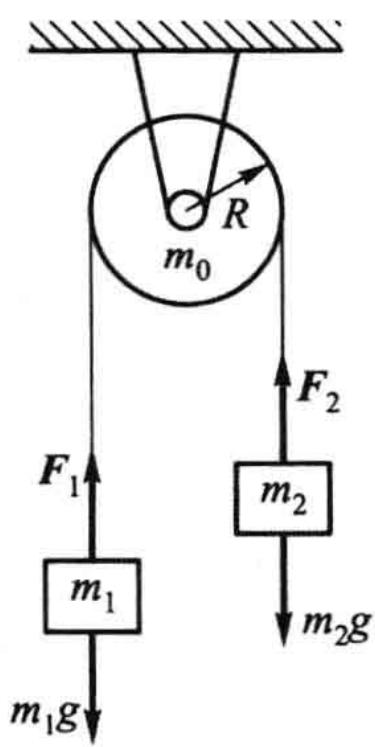
\includegraphics[width=0.18\textwidth]{figures/fig7-19.jpg}
  \end{figure}

\vfill

\textbf{7-20.}同一平面内的半径分别为 $R_{1}$ 和 $R_{2}$ , 质量分别为 $m_{1}$ 和 $m_{2}$ 的轮子以皮带相连接, 可绕各自的轴转动, 如习题 7-20 图所示。今在 $m_{1}$ 轮上作用一力矩 $M$ , 试求两轮的角加速度。设两轮的质量均集中在轮边, 皮带与轮之间无滑动, 皮带的质量和两轴承处的摩擦均可忽略。

\begin{figure}[H]
  \centering
  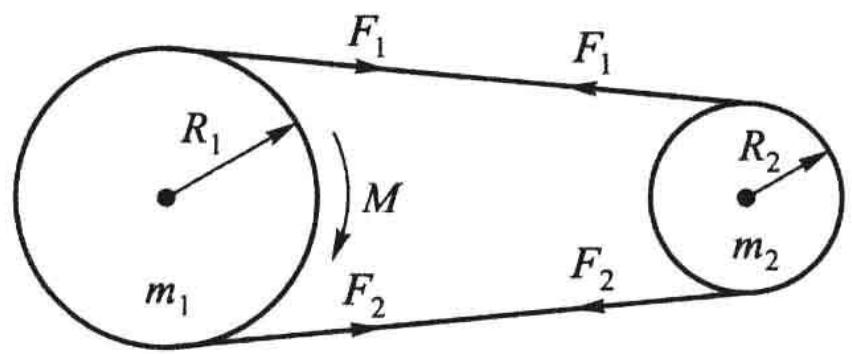
\includegraphics[width=0.35\textwidth]{figures/fig7-20.jpg}
  \end{figure}

\vfill
\newpage

\textbf{7-21.}一质量为 $m_{2}$ 、半径为 $R_{2}$ 的圆盘, 沿着绕在它边缘上的带子展开, 带子跨过一质量为 $m_{1}$ 、半径为 $R_{1}$ 的定滑轮, 带子的另一端悬挂一质量为 $m$ 的重物, 如习题 7-21 图所示。设圆盘沿竖直线下落, 假定皮带的质量可忽略。试求:

(1) 重物 m 的加速度 $a_{1}$ ;

(2) 圆盘质心的加速度 $a_{2}$ 。

\vfill

\textbf{7-22.}如习题 7-22 图所示, 一圆柱体沿倾角为 $\theta$ 的斜面滚下, 圆柱体与斜面之间的摩擦因数为 $\mu$ 。为使圆柱体沿斜面做纯滚动，试求 $\theta$ 的最大值。

\begin{figure}[H]
  \centering
  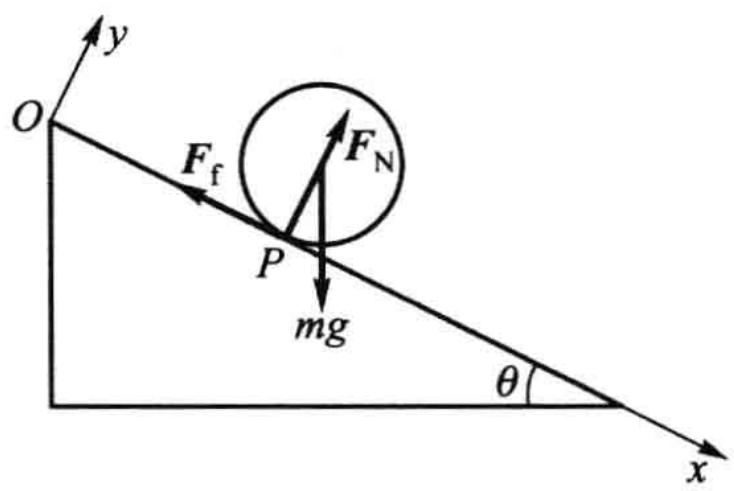
\includegraphics[width=0.3\textwidth]{figures/fig7-22.jpg}
  \end{figure}

\vfill
\newpage

\textbf{7-23.}如习题 7-23 图所示, 在倾角为 $\theta$ 的斜面上, 一质量为 $m$ 、半径为 $r$ 的圆柱体上绕有细绳,绳的一端缠绕在斜面顶端的定滑轮上,定滑轮为一质量为 $m_{0}$ 、半径也为 r 的圆盘。设圆柱体沿斜面滚下时细绳拉直且不能伸长,并与斜面平行,细绳与圆柱体及定滑轮之间无相对滑动,忽略滑轮轴承处的摩擦。

(1) 若圆柱体的滚动为纯滚动, 求其质心的加速度;

(2) 求圆柱体做纯滚动的条件。

\begin{figure}[H]
  \centering
  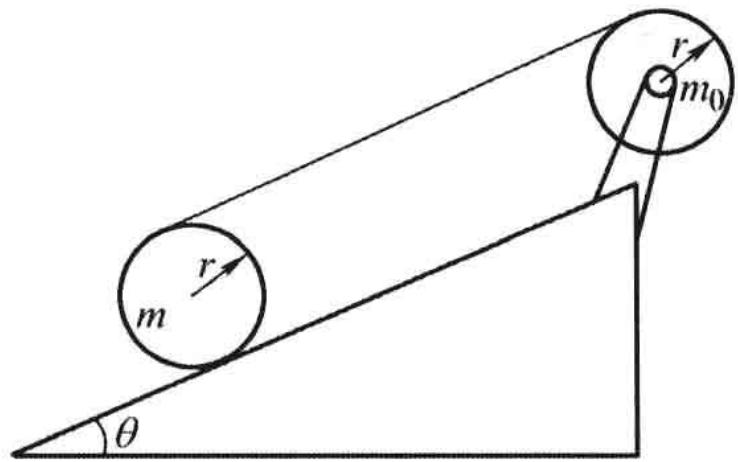
\includegraphics[width=0.3\textwidth]{figures/fig7-23_2.jpg}
  \end{figure}

\vfill

\textbf{7-24.}一质量为 $m_{0}$ , 半径为 $R$ 的均质圆盘, 可绕过其圆心且与盘面垂直的竖直轴自由转动。圆盘原来静止, 盘边上一质量为 $m$ 的人以恒定的相对于盘面的速度 $u$ 沿盘边缘行走时, 盘的转动角速度为多大?

\vfill
\newpage

\textbf{7-25.}一块半径为 $R$ 的水平轻质圆盘, 可绕过其圆心 $O$ 的竖直轴自由旋转。在圆盘下面的边缘处等间隔地系有四个质量都为 m 的小球, 如习题 7-25 图所示。开始时, 圆盘静止, 一辆质量也为 m 的玩具汽车从 O 出发, 以恒定的相对于盘的速率 $v_{0}$ 沿半径驶往盘边, 并沿盘边行驶。试求:

（1）当玩具汽车沿半径行驶时，圆盘的转动角速度 $\omega_{1}$ ;

(2) 当玩具汽车沿盘边行驶时, 圆盘的转动角速度 $\omega_{2}$ 。

\begin{figure}[H]
  \centering
  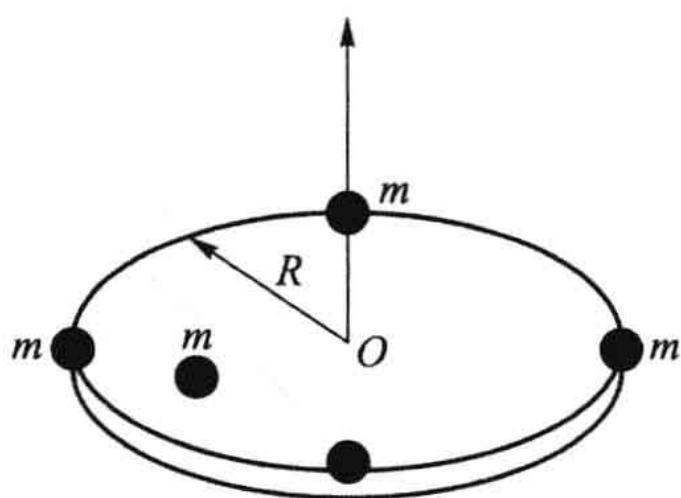
\includegraphics[width=0.25\textwidth]{figures/fig7-25_2.jpg}
  \end{figure}

\vfill

\textbf{7-26.}若上题中的竖直轴不在圆心, 而在某一小球位置处。玩具汽车从该轴处以恒定的相对于圆盘的速率 $v_{0}$ 沿盘边行驶。试求：

(1) 当玩具汽车行驶到第三小球位置处(即行驶了半圈)时,圆盘的转动角速度 $\omega_{1}$ ;

(2) 当玩具汽车行驶到第四小球位置处 (即行驶了 3/4 圈时), 圆盘的转动角速度 $\omega_{2}$ ;

(3) 当玩具汽车回到转轴处时, 圆盘的转动角速度 $\omega_{3}$ 。

\begin{figure}[H]
  \centering
  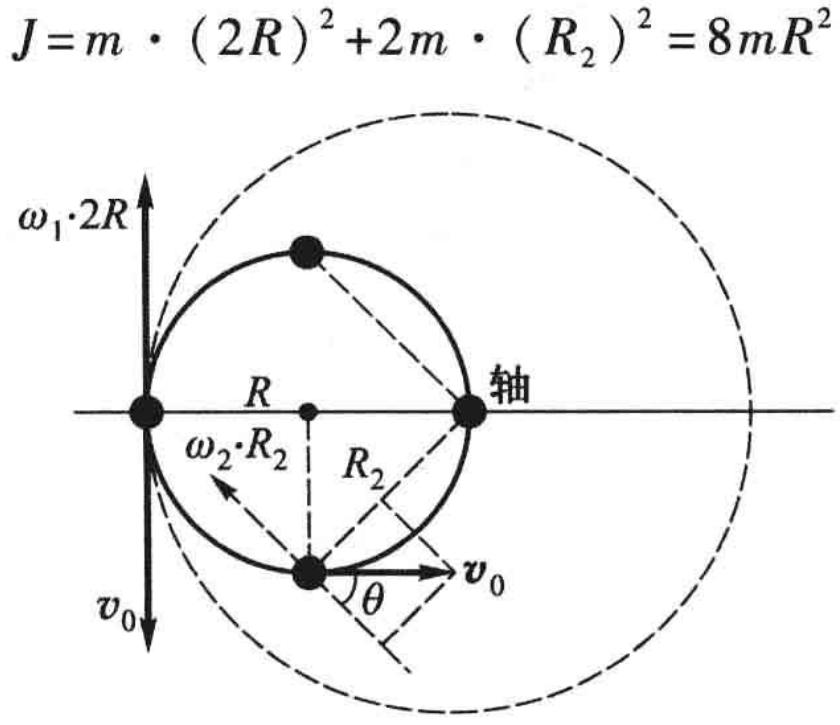
\includegraphics[width=0.3\textwidth]{figures/fig7-26_1.jpg}
  \end{figure}

\vfill
\newpage

\textbf{7-27.}质量皆为 $m$ 的两珠子可在光滑轻杆上自由滑动, 杆可在水平面内绕过 $O$ 点的光滑竖直轴自由旋转。原先两珠对称地位于 $O$ 点的两边, 与 $O$ 相距 $a$ , 在 $t = 0$ 时刻, 对杆施以冲量矩, 使杆在极短时间内即以角速度 $\omega_0$ 绕竖直轴旋转, 求 $t$ 时刻杆的角速度 $\omega$ 、角加速度 $\alpha$ 及两珠与 $O$ 点的距离 $r$ 。

\vfill

\textbf{7-28.}质量为 $m_{0}$ 、长为 $l$ 的均质细棒以一端为支点悬挂起来。一质量为 $m$ 的子弹以 $v_{0}$ 的水平速度射入棒的另一端，且留在棒内。试求在子弹射入棒后，棒的最大偏转角 $\theta$ 。设在棒偏转时，支点处的摩擦可忽略。

\vfill
\newpage

\textbf{7-29.}在一根长为 $3l$ 的轻杆上打一个小孔, 孔离一端的距离为 $l$ , 再在杆的两端以及距另一端为 $l$ 处各系一质量为 $m_0$ 的小球。然后通过此孔将杆悬挂于一光滑的水平细轴 $O$ 上, 如习题 7-29 图所示。开始时, 轻杆静止, 一质量为 $m$ 的小铅粒以 $v_0$ 的水平速度射入中间的小球, 并留在里面。若铅粒相对小球静止时杆的角位移可以忽略, 试求杆在以后摆动中的最大摆角。

\begin{figure}[H]
  \centering
  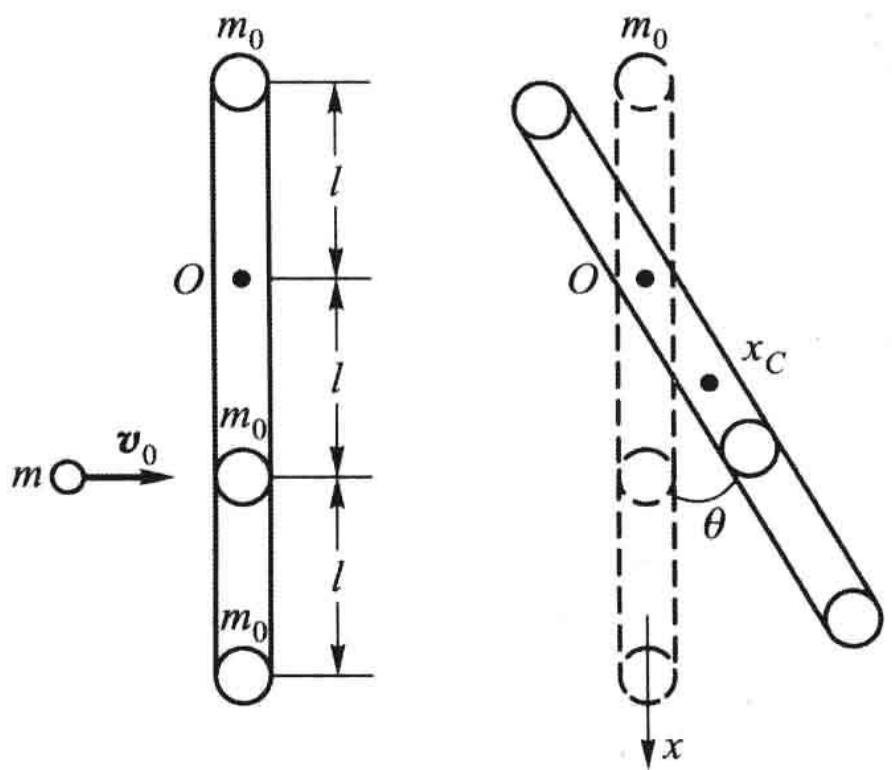
\includegraphics[width=0.3\textwidth]{figures/fig7-29.jpg}
  \end{figure}

\vfill

\textbf{7-30.}将一根长 $l$ 、质量为 $m_0$ 的均匀杆的一端搁在桌边, 另一端用手托住, 使杆处于水平位置, 如习题 7-30 图所示。试求将手释放瞬间杆对桌边的作用力。

\begin{figure}[H]
  \centering
  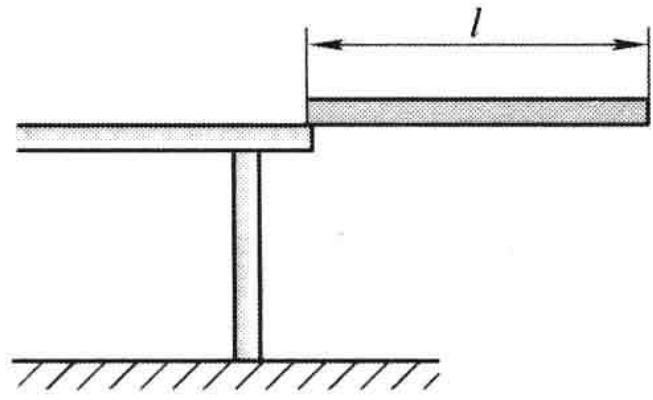
\includegraphics[width=0.3\textwidth]{figures/fig7-30.jpg}
  \end{figure}

\vfill
\newpage

\textbf{7-31.}两根质量均为 $m$ 、长均为 $l$ 的相同均匀杆，与一竖直轴刚性相连，杆与轴均成 $\theta$ 角,且三者在同一平面内,转轴被轴承在 A、B 点处固定,如习题 7-31 图所示。当转轴以恒定角速度 $\omega$ 转动时,求转轴对轴承的水平作用力。设两轴承到杆、轴连接点的距离均为 R。

\begin{figure}[H]
  \centering
  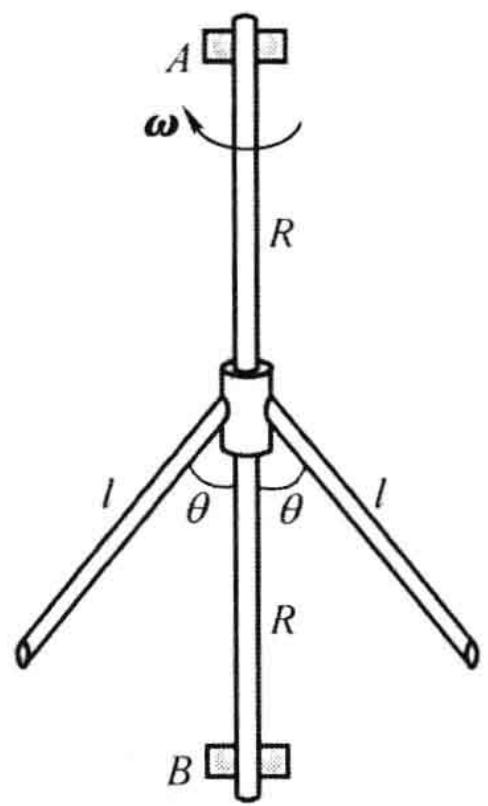
\includegraphics[width=0.2\textwidth]{figures/fig7-31.jpg}
  \end{figure}

\vfill

\textbf{7-32.}一直角尺由长度分别为 $a$ 和 $b$ 的两根棒构成, 能在竖直平面内绕过直角顶点的光滑水平轴自由转动,如习题7-32图所示。设长为 a 的棒与竖直线间的夹角为 $\alpha$ 。开始时,将尺拉至 $\alpha=0$ 位置,然后由静止开始释放。求 $\alpha$ 的最大值。

\begin{figure}[H]
  \centering
  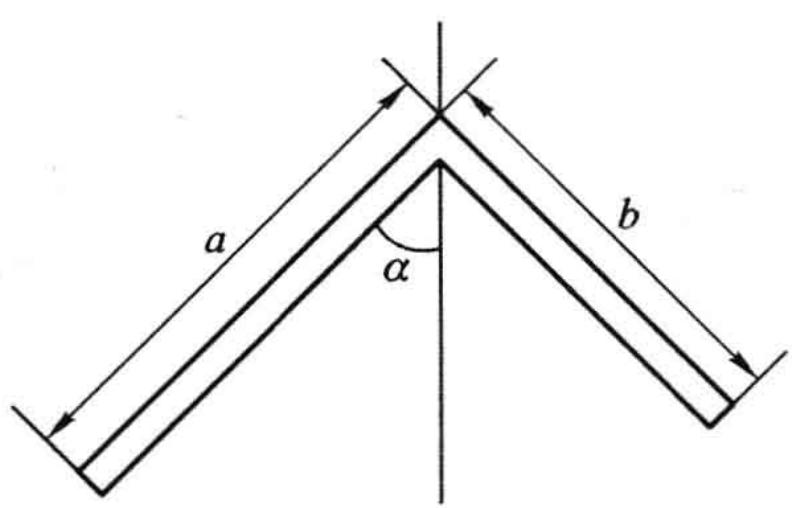
\includegraphics[width=0.3\textwidth]{figures/fig7-32.jpg}
  \end{figure}

\vfill
\newpage

\textbf{7-33.}质量为 $m$ 的板受水平力 $F$ 的作用沿水平面运动, 板与水平面之间的摩擦因数为 $\mu$ 。板上放着质量为 $m_{0}$ 、半径为 $R$ 的圆柱体, 如习题 7-33 图所示。

(1) 若圆柱体在板上的运动为纯滚动, 求板的加速度。

(2) 为使圆柱体做纯滚动, 求 $F$ 的最大值。设圆柱体与板之间的摩擦因数也是 $\mu$ 。

\begin{figure}[H]
  \centering
  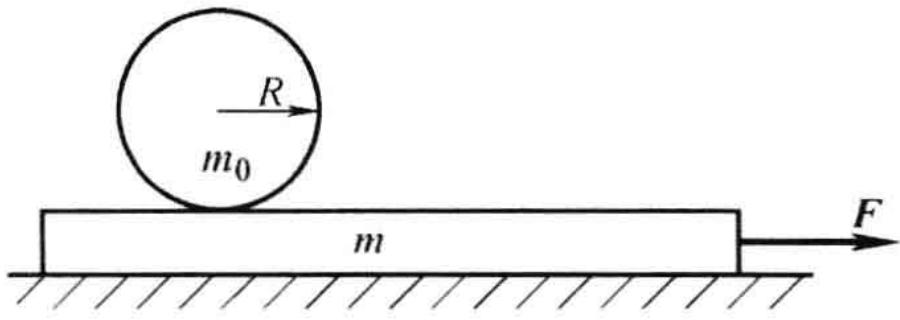
\includegraphics[width=0.4\textwidth]{figures/fig7-33_1.jpg}
  \end{figure}

\vfill

\textbf{7-34.}一根长为 $l$ 、质量为 $m$ 的均匀细棒, 放置在光滑的水平桌面上, 一个水平的冲量 $I$ 突然垂直地作用于棒的另一端。试问:

(1) 当棒旋转了 $360^{\circ}$ 时, 其质心运动了多远?

(2) 冲击后棒的动能为多大?

\vfill
\newpage

\textbf{7-35.}如习题 7-35 图所示, 一质量为 $m$ 、半径为 $r$ 的小球, 从高为 $h_0$ 的斜坡顶端由静止开始滚下, 并从高为 $h(h < h_0)$ 的斜坡的另一端飞离。离开时, 小球的速度为竖直向上, 若小球与斜坡之间的摩擦因数足够大, 使小球始终做纯滚动, 求小球飞离后所能上升的最大高度。

\begin{figure}[H]
  \centering
  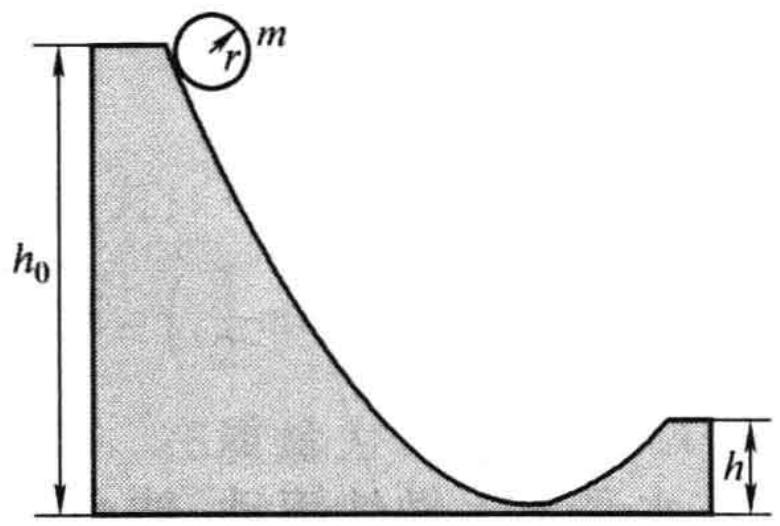
\includegraphics[width=0.3\textwidth]{figures/fig7-35.jpg}
  \end{figure}

\vfill

\textbf{7-36.}将一水平方向上的冲量 $I$ 作用在质量为 $m_{0}$ 、半径为 $R$ 的最初是静止的均质小球上, 作用点位于球心的上方, 距地面的高度为 $h$ , 作用线位于过球心而平行于纸面的平面内, 如习题 7-36 图所示。试分析小球以后的运动情况, 并

求出小球做纯滚动时的角速度 $\omega$ 。

\vfill
\newpage

\textbf{7-37.}一质量为 $m$ 、半径为 $r$ 的均质球 1 在水平面上做纯滚动, 球心速度为 $v_{0}$ , 与另一完全相同的静止球 2 发生对心碰撞, 如习题 7-37 图所示。设碰撞时各接触面间的摩擦均可忽略, 碰撞是弹性的。

（1）碰撞后，各自经过一段时间，两球开始做纯滚动，求出此时各球心的速度；

(2) 求此过程中系统机械能的损失。

\begin{figure}[H]
  \centering
  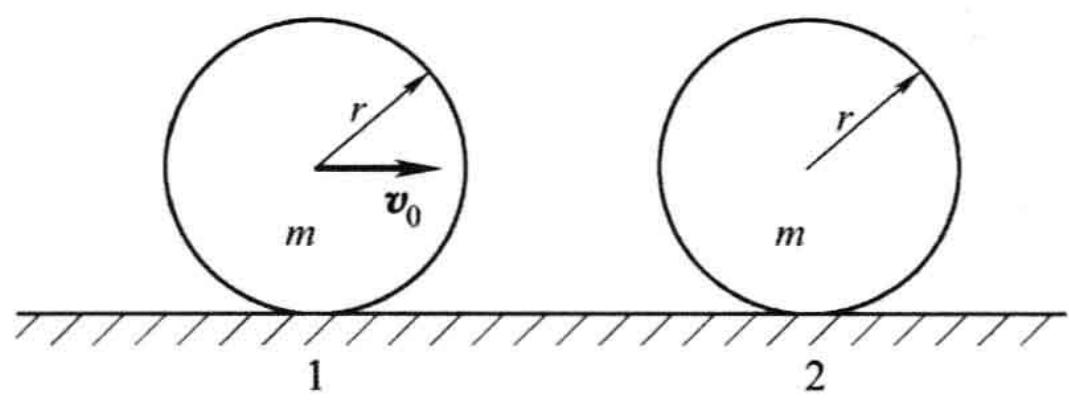
\includegraphics[width=0.35\textwidth]{figures/fig7-37.jpg}
  \end{figure}

\vfill

\textbf{7-38.}在质量为 $m$ 、边长为 $a$ 的正方形板的一个顶点上系一根绳, 绳的长度也是 $a$ , 其另一端与光滑墙面相连。把板的另一顶点靠在墙上, 使绳与板平面处在同一与墙面垂直的竖直平面内, 如习题 7-38 图所示。求平衡时绳中的张力。

\begin{figure}[H]
  \centering
  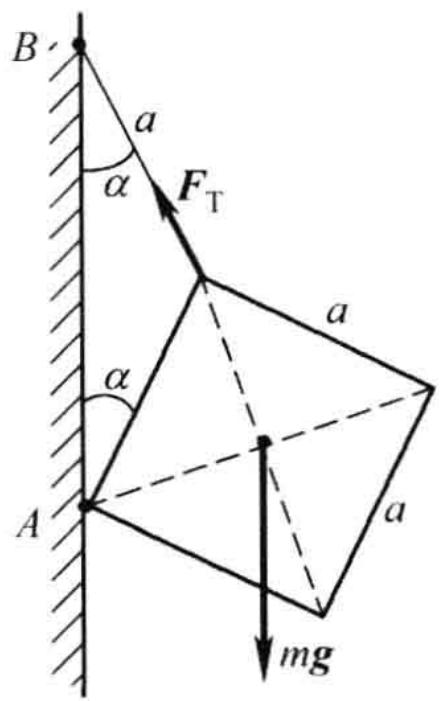
\includegraphics[width=0.2\textwidth]{figures/fig7-38.jpg}
  \end{figure}

\vfill
\newpage

\textbf{7-39.}质量为 $m$ 的线轴如习题 7-39 图所示, 其外半径为 $a$ , 绕线部分的半径为 $b$ , 设其绕轴线的转动惯量为 $J$ 。今将绕线的一端以一恒力 $F$ 拉它, $F$ 与水平面成 $\theta$ 角, 设 $F \sin \theta < mg$ 。

(1) 为使线轴向后 (即与 $F$ 的水平分量方向相反) 做纯滚动,

(i) 求 $\theta$ 的范围；

(ii) 若满足(i)中的条件,则摩擦因数 $\mu$ 至少应为多大?

(iii) 求出线轴质心运动的加速度。

(2) 为使线轴向前做纯滚动, 同样求出 (1) 中的三个问题。

\vfill

\textbf{7-40.}一质量为 $m$ 、半径为 $R$ 的圆盘可绕通过其中心 $O$ 的竖直轴以 $\omega$ 角速度转动,如习题7-40图所示。试求轴承处所受的水平作用力,设OA=OB=l,垂直于圆盘表面的法线与竖直轴成 $\alpha$ 角。

\begin{figure}[H]
  \centering
  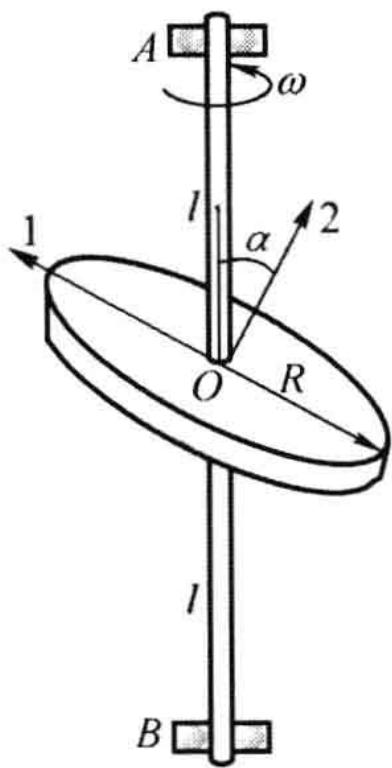
\includegraphics[width=0.2\textwidth]{figures/fig7-40.jpg}
  \end{figure}

\vfill
\newpage

\textbf{7-41.}如习题 7-41 图所示,一陀螺由一质量为 $m$ 、半径为 $R$ 的厚圆盘构成,通过圆心且垂直于圆盘的自转轴为一轻杆,杆的尖端自由地支在离盘质心为 l 处的枢纽上。现陀螺绕自转轴以 $\omega_{0}$ 的角速度高速自转,其自转轴以与水平面成 $\theta$ 角做均匀进动。试求:(1) 进动角速度;(2) 枢纽所受的力。

\begin{figure}[H]
  \centering
  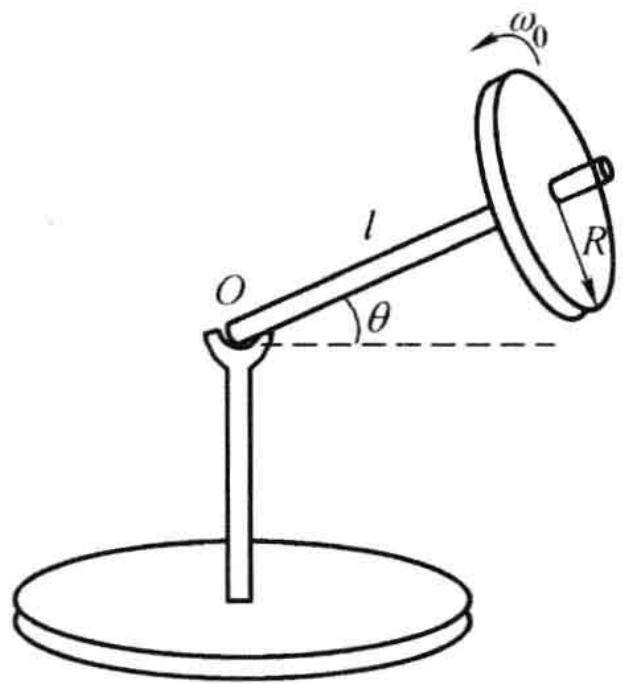
\includegraphics[width=0.25\textwidth]{figures/fig7-41.jpg}
  \end{figure}

\vfill

\textbf{7-42.}一半径为 $r$ 的硬币,在桌面上绕半径为 $R$ 的圆滚动,其质心速度为 $v$ , 如习题 7-42 图(a)所示。设硬币的滚动为纯滚动。求其轴线与水平线所成的角 $\theta(\theta<<1,R>>r)$ 。

\begin{figure}[H]
  \centering
  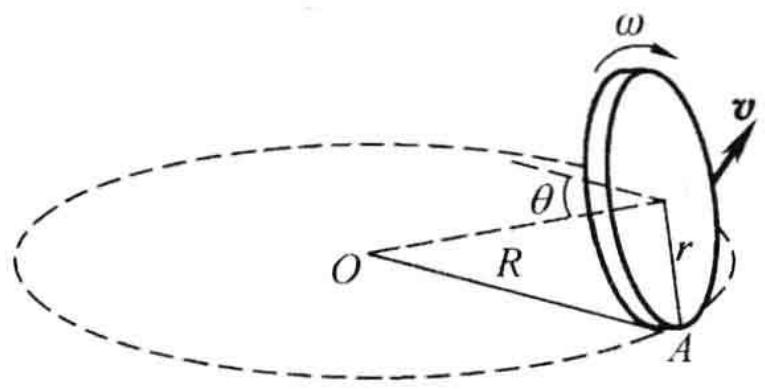
\includegraphics[width=0.3\textwidth]{figures/fig7-42_a.jpg}
  \end{figure}

\vfill
\newpage

\textbf{7-43.}一陀螺由半径为 $R$ 、质量为 $m$ 的薄圆盘及过其圆心且垂直于盘面的轻杆组成, 盘缘及杆的一端 $O$ 靠在桌面上, 杆与桌面成 $45^{\circ}$ 角, 如习题 7-43 图 (a) 所示。今陀螺以杆的一端 $O$ 为支点, 靠在桌面上做无滑滚动, 使杆绕竖直轴做匀速转动, 角速度为 $\Omega$ 。求:

(1) 桌面对盘缘的支承力 $F_{N}$ ;

(2) 陀螺的动能。

\begin{figure}[H]
  \centering
  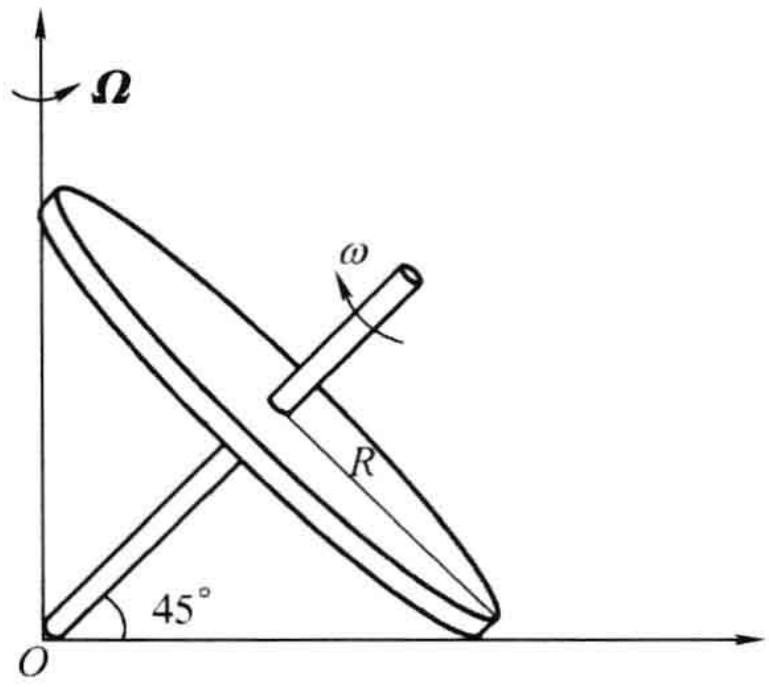
\includegraphics[width=0.3\textwidth]{figures/fig7-43_a.jpg}
\end{figure}

\vfill
\newpage